\documentclass[a4paper,12pt]{article}

% don't forget the document class, generally : \documentclass[a4paper,12pt]{article}

\usepackage[utf8]{inputenc}
\usepackage[french]{babel}
\usepackage{graphicx}
\usepackage{gensymb}
\usepackage{amsmath}
\usepackage{float}
\usepackage{scrextend}
\usepackage{caption} 
\usepackage{siunitx}
\usepackage{enumitem}
\usepackage{amsthm}
\usepackage{fancyhdr}
\usepackage{amssymb}
\usepackage{wrapfig}
\usepackage{geometry}
\usepackage{standalone}
\usepackage{import}
\usepackage[usenames, dvipsnames]{color}

 \usepackage{biblatex} % manages bibliography and references
\addbibresource{sample.bib}


\geometry{hmargin=1in, vmargin=1in}

 \newenvironment{absolutelynopagebreak}
 {\par\nobreak\vfil\penalty0\vfilneg
 \vtop\bgroup}
 {\par\xdef\tpd{\the\prevdepth}\egroup
 \prevdepth=\tpd}
 
 \pagestyle{fancy}                        
\fancyhf{}                               
\fancyhf[HL]{Application des maths}                
\fancyhf[HR]{Géométrie euclidienne}             
\fancyhf[FC]{\thepage/\pageref{Lastpage}}
 
\newtheorem{definition}{Définition}[section]
\newtheorem{theorem}{Théorème}
\newtheorem{corollary}{Corollaire}[theorem]
\newtheorem{lemma}[theorem]{Lemme}
\newtheorem*{hyp}{Hypothèse}
\newtheorem*{concl}{Conclusion}
\newtheorem*{remark}{Remarque}

\captionsetup{format=default,labelformat=simple,labelsep=colon,
justification=justified,font={sf,small},labelfont=bf,
textfont=default} 



\begin{document}

\pagebreak
\subsection{Théorème de l'intersection des médianes}
Commençons par définir la médiane.
\begin{definition}{Médiane:}
Droite passant par le sommet d'un triangle et qui partage le côté opposé en deux parties égales.
\end{definition}

\begin{theorem}
Les médianes d'un triangle concourent en un point situé à deux tiers des sommets du triangle.
\end{theorem}

\begin{proof}
Nous considérons le triangle quelconque $ABC$ et nous représentons les point $A'$, $B'$ et $C'$ qui coupent les respectivement les côtés $a$, $b$ et $c$ en leurs milieux. 
\begin{hyp}
Les segments $AA'$ et $BB'$ sont confondus avec les médianes du triangle $ABC$, ils se croisent en un point $G$.
\end{hyp}
\begin{concl}
La droite qui passe par les points $C$ et $G$ coupe le segment $AB$ en $C'$.
\end{concl}

Nous construisons un point $L$ sur le prolongement de $CG$ de sorte à ce que $GL \equiv CG$.

\begin{figure}[H]
        \centering
        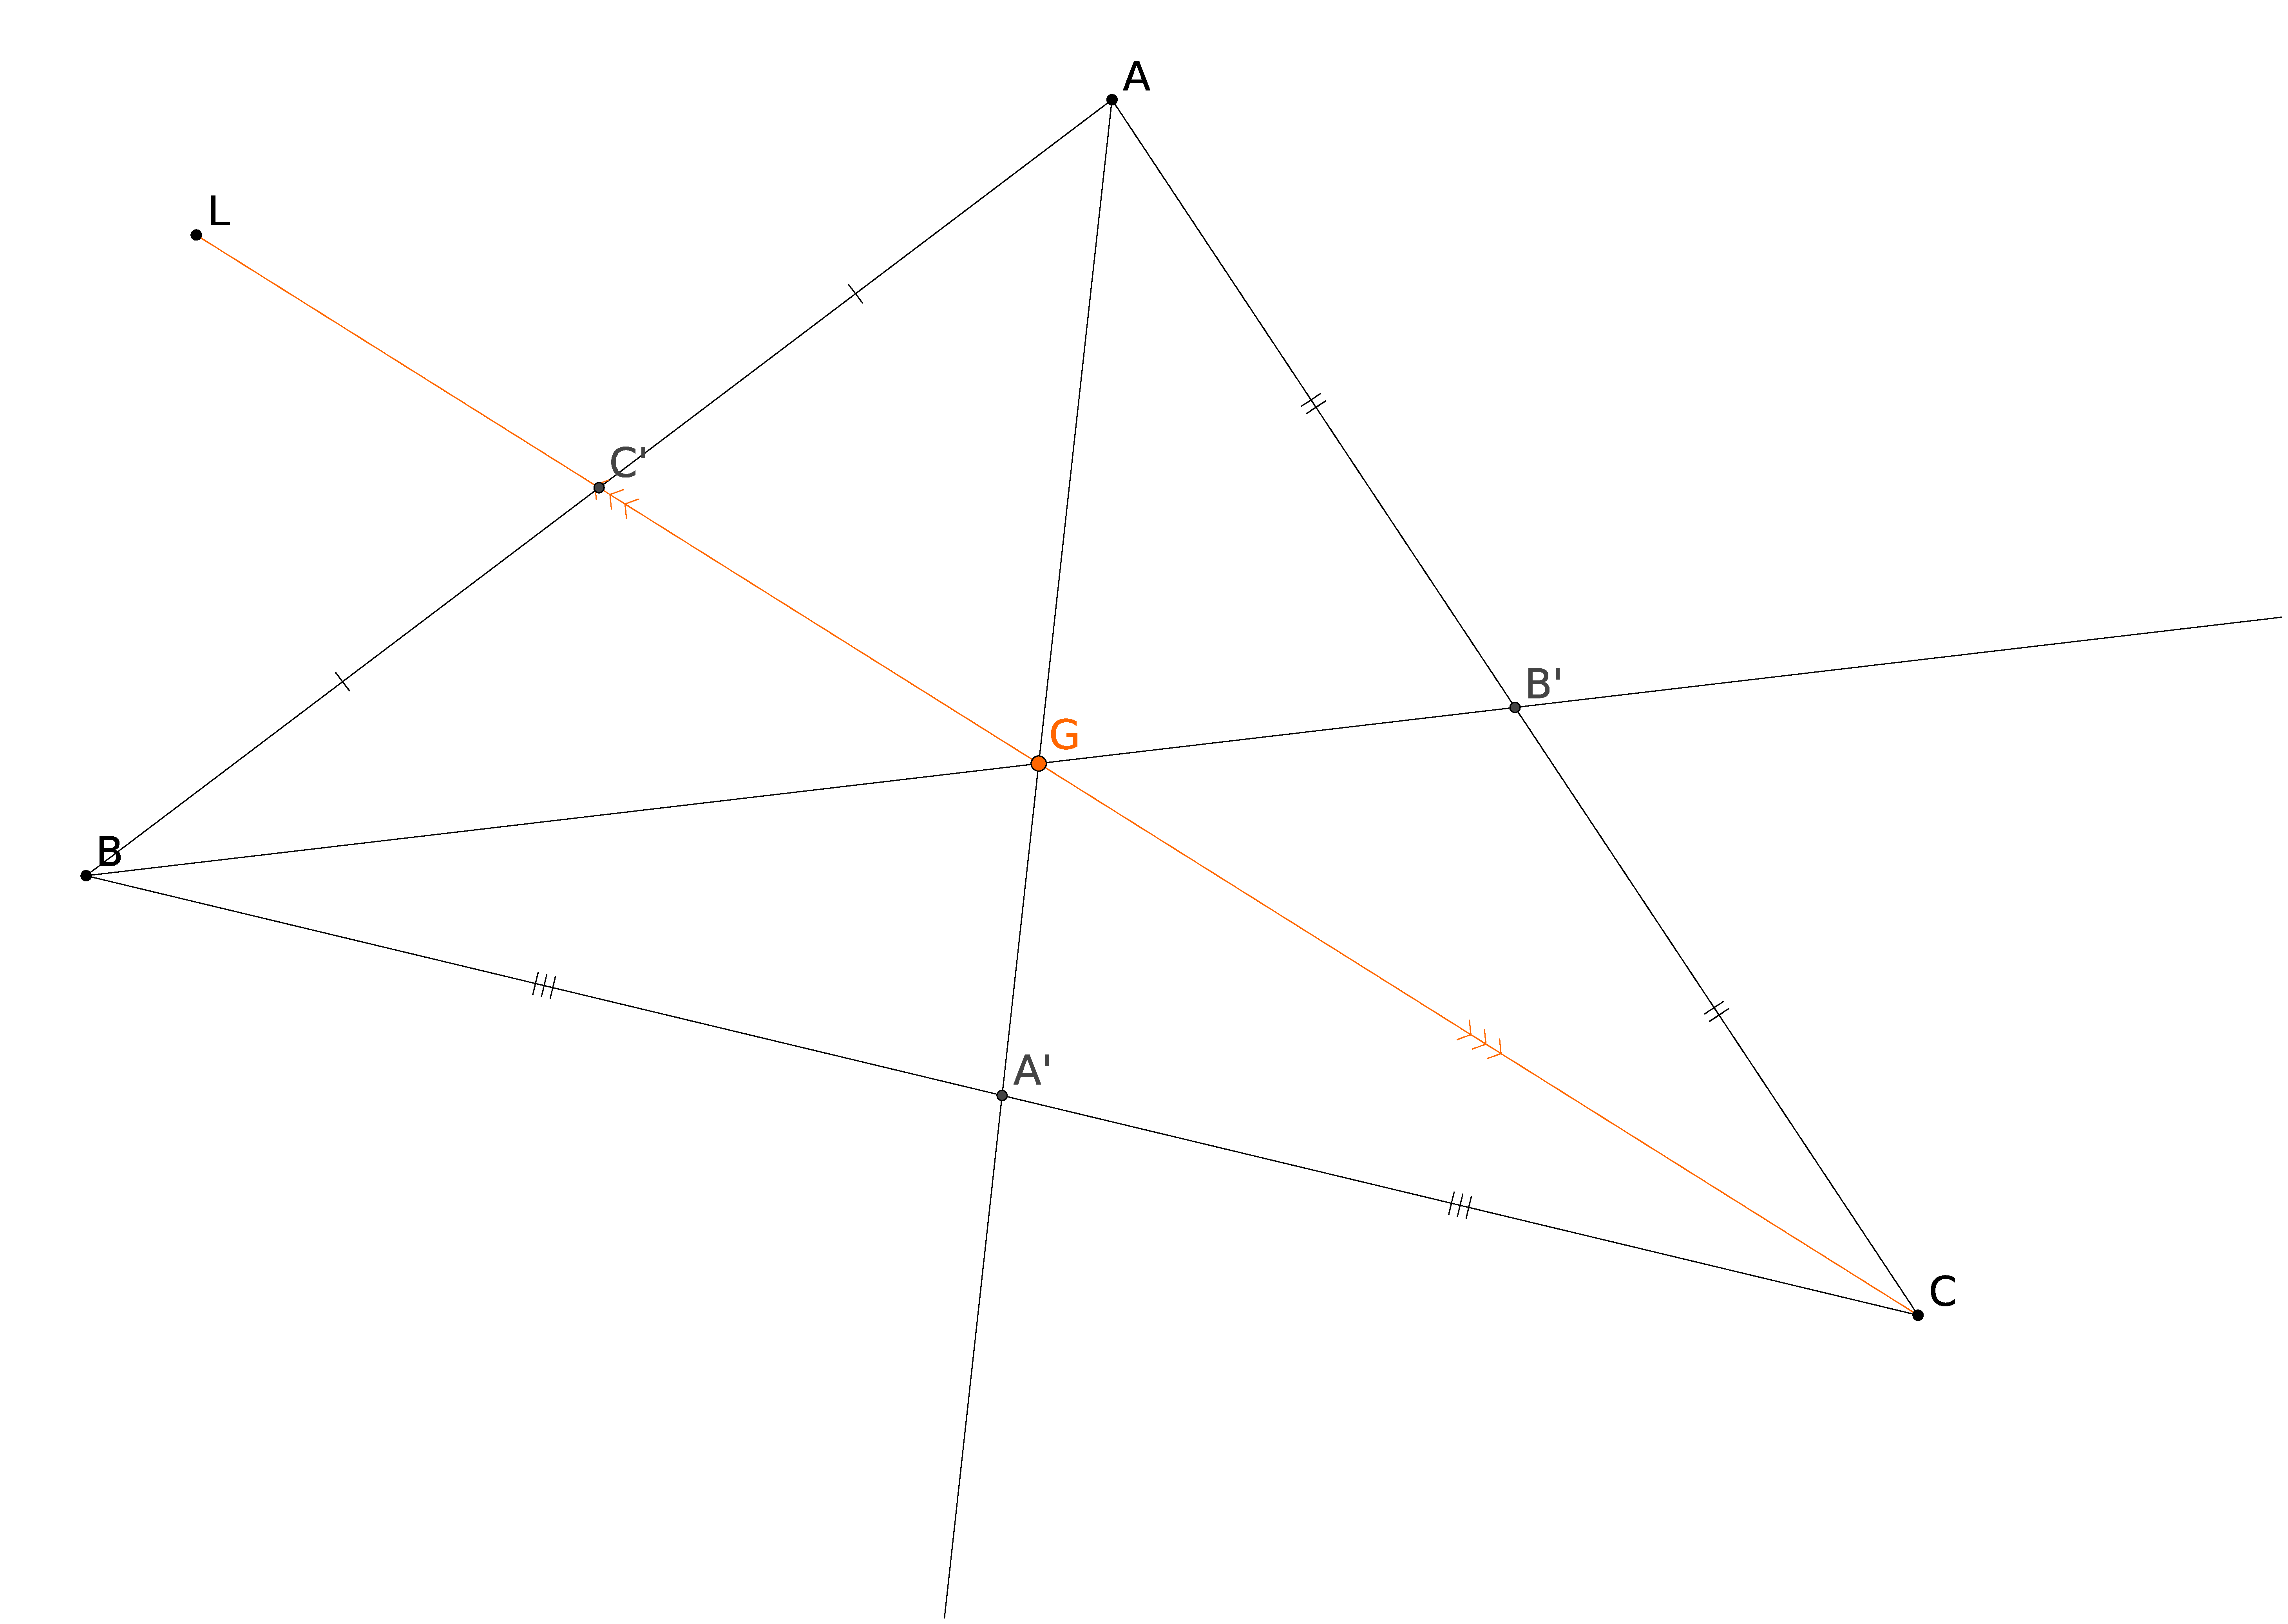
\includegraphics[scale=0.15]{mediane1.eps}
    \end{figure}

Ainsi, nous observons que les segments $GB'$ et $LA$ sont parallèles, car $CG \equiv GL$ et $CB' \equiv B'A$ (voir théorème \ref{semblableTh2}). Les segments $BG$ et $LA$ sont donc parallèles ($BG$ est le prolongement de $GB'$). En suivant le même raisonnement, nous concluons que $BL$ est parallèle à $GA$. 

\begin{figure}[H]
        \centering
        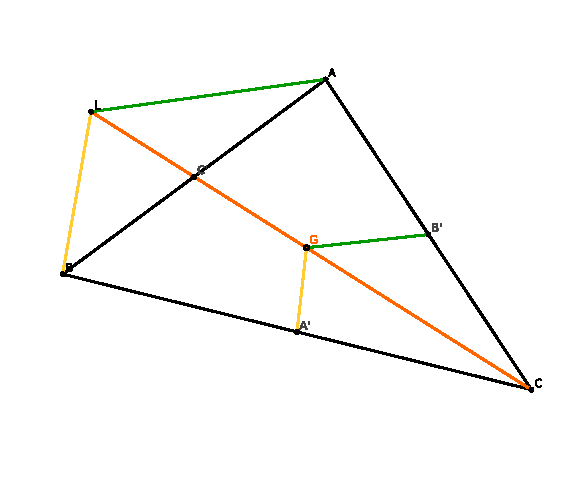
\includegraphics[scale=1.3]{mediane2.eps}
    \end{figure}

Par conséquent le quadrilatère $BLAG$ est un parallèlogramme car il a deux paires de côtés parallèles. Puisque les diagonales des parallèlogrammes se coupent en leurs milieux (théorème \ref{th:parallelogramme}), nous savons que $BC' \equiv C'A$. Cela signifie que la droite qui passe par $CG$ est confondue avec la médiane du triangle $ABC$ passant par $C$.\\

\begin{figure}[H]
        \centering
        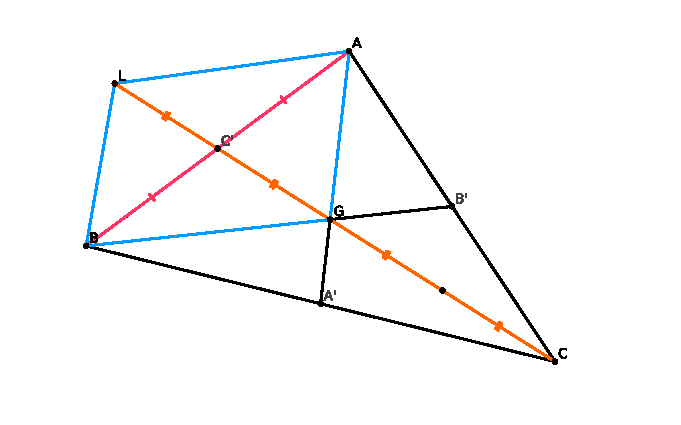
\includegraphics[scale=1.3]{mediane3.eps}
    \end{figure}

De plus, nous observons que $LC \equiv C'G$  et que $CG$ est donc égal à deux $C'G$ et les médianes des triangles se croisent à deux tiers de de leurs sommets.
\end{proof}
\end{document}